\documentclass[10pt,letterpaper]{article}
\usepackage[T1]{fontenc}
\usepackage{amssymb}
\usepackage{amsmath}
\usepackage{enumerate}
\usepackage[margin=0.5in]{geometry}
\usepackage{graphicx}
\usepackage{siunitx}
\usepackage{wrapfig}
\usepackage{xcolor}
\title{Introduction to Quantum Electronic Devices and Applications}
\author{Jeremy Chen}
\date{03/10/2026}
\begin{document}
	\maketitle
	
\begin{enumerate}[\textbf{\arabic{enumi}.}]

\item \textbf{Spherical Quantum Dots}

Due to the tunability of their energy levels, spherical quantum dots (QD) are used in a variety of optical applications. The spacing between their energy levels determines the wavelengths they absorb and emit, allowing QDs to be engineered to convert higher-energy light (typically blue, around $\lambda \approx 450$nm) into lower-energy light (such as green or red). This property is useful in “white light LEDs”, where layers of red- and green-emitting QDs are placed on top of a blue-emitting LED. The resulting combination of wavelengths produces a spectrum that spans much of the visible spectrum and appears yellow or white.

\begin{figure}[h!]
\centering
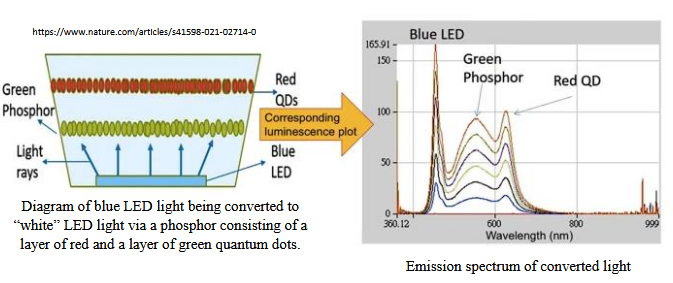
\includegraphics[width=0.9\linewidth]{Phosphor.png}
\end{figure}

In this problem, we'll design QDs that emit radiation at green and red wavelengths.

\begin{enumerate}[a)]

\item We first need to determine the energy levels of a spherical quantum dot, which we’ll model using the following potential
$$V(r) = \begin{cases}
0, & \text{for  } r \leq a \\
\infty, & \text{for  } r > a'
\end{cases}$$
where $a$ is the radius of the quantum dot. From lecture, we know that the stationary states of the Schrödinger equation in a central potential are of the form
$$\psi(r, \theta, \varphi) = Y_{l}^{m}(\theta, \varphi)R(r)$$
where $Y_{l}^{m}$ are the normalized spherical harmonics and $R(r)$ must be determined for our specific potential. Inside our QD, where $V(r) = 0$, we have the following radial equation to solve:
$$\frac{d^{2}u}{dr^{2}} = \left[ \frac{l(l + 1)}{r^{2}} - k^{2} \right]u, \text{ where } u(R) = rR(r) \text{ and } k = \sqrt{2mE}/\hbar$$
Again, this is a known differential equation and the solutions are \textit{spherical Bessel functions} ($j_l$) and \textit{spherical Neumann functions} ($n_{l}$):
$$R(r) = Aj_{l}(kr) + Bn_{l}(kr), \text{ where } l = 0, 1, 2, 3, \dots$$
and $j_{l}(r) \propto r^{l}$ and $n_{l}(r) \propto \frac{1}{r^{l + 1}}$. To find our energies, we need to apply boundary conditions. 

\begin{enumerate}[i)]

\item \textit{Condition \#1}: the wave function must be normalizable, requiring that it be finite on the domain $0 \leq r \leq \infty$. What does this condition require in terms of the constants A and/or B?

\color{violet}
The constants $A$ and $B$ must be the solutions to the Bessel and Neumann functions. This is given by Abel's identity. 
\color{black}

\item \textit{Condition \#2}: the wave function $R(r)$ must vanish at $r = a$ since the potential there is $\infty$. What constraint does this place on the quantity $kr$? \textit{Hint}: at what values fo $kr$ is $R$ zero?

\color{violet}
It depends on the root of the function, or the roots for $J_{n + \frac{1}{2}}(kr)$, so $kr$ could not ever 
\color{black}

\item Show that the expression for the energy levels in the spherical QD is
$$E_{n, l} = \frac{\hbar^{2}}{2ma^{2}}\zeta_{n, l}^{2}$$
where $\zeta_{n, l}$ is the $n^{th}$ zero of the $l^{th}$ order spherical Bessel function.

\color{violet}

\color{black}

\end{enumerate}

\item Next, we need to determine the required energy level spacings for emitting radiation at the desired wavelengths. Our QDs should emit radiation at $\lambda = 530$nm for green QDs and $\lambda = 620$nm for red QDs. What energy spacings (in eV) correspond to each of those wavelengths?

\color{violet}
Given the wavelengths, the energy spacing could be determined with $E = \frac{hc}{f}$. For green light, the energy the photon has is
$$E = \frac{\num{6.626e-34} * \num{3e8}}{\num{530e-9}} = \num{3.751e-19}\text{ J} = 2.341\text{ eV}$$
and the energy for a red photon is
$$E = \frac{\num{6.626e-34} * \num{3e8}}{\num{620e-9}} = \num{3.206e-19}\text{ J} = \num{2.001}\text{ eV}$$
\color{black}

\item Finally, we will choose material systems for our QDs and the appropriate radius $a$ to achieve the energy spacings above. Similar to Homework 4 Problem 1, the energy of the photon that will be emitted by the QD is given by $E_{photon} = E_{g} + 2E_{gs}$, where $E_{g}$ is the bandgap energy of the QD material and $E_{gs}$ is the ground state energy of the QD as illustrated below.

\begin{figure}[h!]
\centering
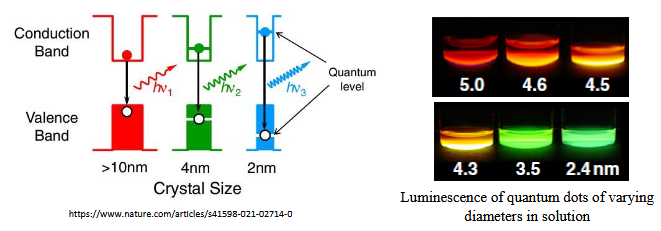
\includegraphics[width=0.9\linewidth]{Bands.png}
\end{figure}

\textit{Note}: the first spherical Bessel function zero is given by $\zeta_{1.0} = \pi$. 

\begin{enumerate}[i)]

\item Cadmium selenide (CdSe) is a common material for QDs with a band gap energy $E_{g} = 1.74$eV and effective electron mass $m_{e} = 0.13m_{0}$. What radius $a$ would give the appropriate energy spacing for emitting green light at $\lambda = 530$nm?

\color{violet}
Given that the energy of a green photon is calculated to be $2.341$ eV, the $E_{gs}$ of a green photon must be $(2.341 - 1.74)/2 = 0.301\text{ eV} = \num{4.815e-20}$ J, and when evaluated for the expression for energy levels, gets
\begin{gather*}
E_{n, l} = \frac{\hbar^{2}}{2ma^{2}}\zeta_{n, l}^{2} \rightarrow a = \sqrt{\frac{\hbar^{2}}{2mE_{n, l}}\zeta_{n, l}^2} \rightarrow \sqrt{\frac{(\num{1.055e-34})^{2}}{2 * 0.13 * \num{9.109e-31} * \num{4.815e-20}}\pi^{2}} = \num{3.104e-9}\text{ m}
\end{gather*}
or $3.104$ nm. 
\color{black}

\item Lead sulfide (PbS) is also a common material for QDs. Its bandgap energy $E_{g}$ is 0.37eV and the mass of its electrons is $m_{e} = 0.105m_{0}$. What radius $a$ would give the appropriate energy spacing for emitting red light at $\lambda = 620$nm?

\color{violet}
Same process as the previous question is used here, $2E_{gs}$ of a red photon is $0.816$ eV or $\num{1.307e-19}$ J. The radius of the QDs should then be
\begin{gather*}
a = \sqrt{\frac{(\num{1.055e-34})^{2}}{2 * 0.105 * \num{9.109e-31} * \num{1.307e-19}}\pi^{2}} = \num{2.096e-9}\text{ m}
\end{gather*}
or $2.096$ nm. 
\color{black}

\end{enumerate}

\end{enumerate}

\item \textbf{Hydrogen-like Atoms}

A major class of quantum computers, trapped-ion quantum computers, uses ions held in an oscillating electromagnetic field as qubits. These ions consist of a single valence electron bound to a nuclear core containing protons, neutrons, and inner-shell electrons. One commonly used example is the $\text{Ca}^{+}$ (or Calcium-40) ion, which has 20 protons and 20 neutrons in the core, 18 electrons in the inner shells, and one valence electron:

\begin{figure}[h!]
\centering
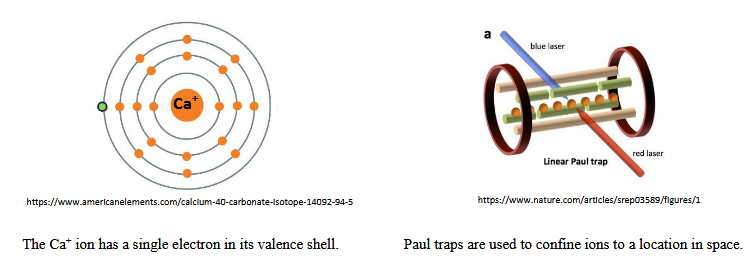
\includegraphics[width=0.8\linewidth]{Trapped Ion.png}
\end{figure}

In this problem, we will derive the energy levels and wave functions for hydrogen-like ions and begin to explore how these ions can be used as qubits.

\begin{enumerate}[a)]

\item The primary difference between the hydrogen atom and hydrogen-like ions is that the hydrogen atom has only one proton in the nucleus with charge $q = e$, whereas hydrogen-like ions have $Z$ protons (the element's atomic number), giving the nucleus a total charge $q = Ze$. As a result, the angular wave functions $Y_{l}^{m}(\theta, \varphi)$ remain the same as for the hydrogen atom, but the radial equation becomes
$$-\frac{\hbar^{2}}{2m_{e}} \frac{d^{2}u}{dr^{2}} + \left[ -\frac{Ze^{2}}{4\pi\epsilon_{0}r} \frac{1}{r} + \frac{\hbar^{2}}{2m_{e}}\frac{l(l + 1)}{r^{2}} \right]u = Eu$$
Determine the following for hydrogen-like ions by making the substitution $e^{2} \rightarrow Ze^{2}$:

\begin{enumerate}[i)]

\item the ground state wave function $\psi_{1, 0, 0}(r, \theta, \varphi)$

\color{violet}
Given that for a hydrogen atom $\kappa = \left( \frac{m_{e}e^{2}}{4\pi\epsilon_{0}\hbar^{2}} \right)\frac{1}{n}$, and that $\kappa$ is derived from $\rho_{0}$, for a hydrogen-like ion, $\kappa = \frac{m_{e}Ze^{2}}{4\pi\epsilon_{0}\hbar^{2}}\frac{1}{n}$. 
\color{black}

\item the Bohr radius $a_{z}$

\color{violet}
The Bohr radius is given by $\kappa = \left( \frac{m_{e}e^{2}}{4\pi\epsilon_{0}\hbar^{2}} \right)\frac{1}{n} = \frac{1}{an}$, so for a hydrogen-like ion the Bohr radius is
$$a \equiv \frac{4\pi\epsilon_{0}\hbar^{2}}{m_{e}Ze^{2}}$$
\color{black}

\item the bound state energies $E_{n}$ for the hydrogen-like ion.

\color{violet}
The energy is determined by $\rho_{0}$, which leads to $E = -\frac{\hbar^{2}\kappa^{2}}{2m_{e}}$. So the allowed energies is given by
$$E_{n} = -\left[ \frac{m_{e}}{2\hbar^{2}} \left( \frac{Ze^{2}}{4\pi\epsilon_{0}} \right)^{2} \right] \frac{1}{n^{2}}$$
\color{black}

\end{enumerate}

\item Qualitatively, what happens to the spread $\sigma_{r}$ of the ground state, the Bohr radius $a_{z}$, and bound state energies $E_{n}$ as $Z$ increases? What is a possible classical explanation for this?

\textit{Hint}: think electrostatic forces!

\color{violet}
As $Z$ increases, $\sigma_{r}$ and $E_{n}$ would both increase, whereas the $a_{z}$ would decrease. The classical explanation would be the increasing number of protons causing more greater attraction on the electron and greater repulsion between protons. 
\color{black}


\item Since our electron is in the valence shell, it is in an excited state rather than the ground state. Given the restrictions on the values of $n$, $l$, and $m$ for the Hydrogen atom and the fact that each state $\{ n, l, m \}$ holds up to two electrons due to spin, determine the principal quantum number $n$ and energy $E_{n}$ of the lone valence electron (the $19^{th}$) of the $\text{Ca}^{+}$ ion

\textit{Hint}: you will need to reference the filling order of atomic orbitals (the Aufbau principle).

\color{violet}
The Aufbau principle gives a general filling order of $n + l$, where orbitals with lower $n + l$ will get filled first. Every state holds up to 2 electrons, so the principle quantum number for the valence electron of the ion should be 4. Given that and the bound state relation, the energy of the ion should be
\begin{gather*}
E_{n} = - \left[ \frac{m_{e}}{2\hbar^{2}} \left( \frac{Ze^{2}}{4\pi\epsilon_{0}} \right)^{2} \right] \frac{1}{16} = -\left[ \frac{\num{9.109e-31}}{2 * (\num{1.055e-34})^2} \left( \frac{20 * (\num{1.602e-19})^2}{4 * \pi * \num{8.854e-12}} \right)^2 \right] \frac{1}{16} = \num{5.442e-17}\text{ J} \\
= -339.754\text{ eV}
\end{gather*}
\color{black}

\item Assuming the valence electron is in level $n$ (for part c), how much energy $\Delta E$ in eV is needed to promote it to level $n + 1$? What frequency $f$ in Hz corresponds to this transition? Is this frequency attainable with current technology?

\color{violet}
At $n + 1$, the ion would have $-217.443$ eV of energy. That is a difference of $-122.311$ eV, or $\num{1.959e-17}$ J. The frequency required for this transition would be $\num{2.957e16}$ Hz, which is achievable, as it lies around the spectrum of UV lights. 
\color{black}

\end{enumerate}

\item \textbf{Gate Current Leakage in MOSFETs (Revisited)}

In Homework 4, we estimated the electron tunneling probability and leakage current density through the MOSFET oxide by modeling the oxide as a rectangular barrier. In actual devices, the potential difference between the semiconductor and the metal gives rise to an electric field $\vec{E}$ inside the oxide layer, producing a trapezoidal barrier, as shown below.

\begin{figure}[h!]
\centering
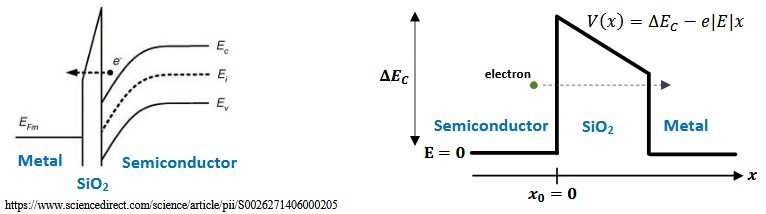
\includegraphics[width=0.9\linewidth]{Trapezoidal Barrier.png}
\end{figure}

We will estimate the tunneling probability and current density through the oxide layer for this trapezoidal barrier using the WKB approximation, then compare this result with what we obtained using the rectangular barrier model in Homework 4.

\begin{enumerate}[a)]

\item First, we'll derive an expression for the tunneling probability of an electron with energy $E_{el}$ through a trapezoidal potential barrier of the form $V(x) = \Delta E_{C} - e|E|x$.

\begin{enumerate}[i)]

\item Write down the WKB expression for the tunneling probability through the trapezoidal barrier in integral form, in terms of $\Delta E_{C}$, $E_{el}$, $|E|$, $x$, and integral limits $x_{0}$ and $x_{1}$.

\color{violet}
The approximate tunneling probability using WKB approximation is $e^{-\frac{2}{\hbar}\int_{x_{0}}^{x_{1}}|p(x)|dx}$, where $p(x) = \sqrt{2m(E_{el} - V(x))} = \sqrt{2m(E_{el} - (\Delta E_{C} - e|E|x))}$. So it would be rewritten as
\begin{gather*}
T = e^{-\frac{2}{\hbar} \int_{x_{0}}^{x_{1}} \sqrt{2m(E_{el} - \Delta E_{C} + e|E|x)}dx}
\end{gather*}
\color{black}

\item Evaluate your integral in part a.i) to obtain an analytical expression for the tunneling probability through the trapezoidal barrier. Leave your answer in terms of $x_{1}$; you will determine a value for $x_{1}$ later.

\color{violet}
Given that $x_{0} = 0$, the analytical expression for the tunneling probability is
\begin{gather*}
T = e^{-\frac{2^{3/2}e^{-1}(m(e|E|L + E_{el} - E_{C}))^{3/2}}{\hbar|E|m}}
\end{gather*}
Setting $\kappa = \frac{2^{3/2}e^{-1}(m(e|E|L + E_{el} - E_{C}))^{3/2}}{2\hbar|E|m}$ to get $T = e^{-2\kappa x_{1}}$, or
\begin{gather*}
T = \frac{1}{1 +  \frac{V_{0}^{2}\sinh^{2}(\kappa x_{1})}{4E_{el}(E_{el} - \Delta E_{C} + e|E|x)}}
\end{gather*}
\color{black}

\end{enumerate}

\item Now we’ll calculate the tunneling probability and current density for the same set of parameters we investigated in Homework 4:

\begin{itemize}

\item Oxide thickness: $t_{ox} = 0.5$ nm 

\item Oxide potential barrier height on the semiconductor side: $\Delta E_{C} = 3.2$ eV

\item Electron energy: $E_{el} = 1.0$ eV

\item Potential difference across the oxide: $V_{0} = 1$ V

\item Current density attempting to tunnel from the semiconductor: $J_{i} = 4.75 \times 10^{10} A/m^{2}$

\end{itemize}

\begin{enumerate}[i)]

\item Assuming that the potential in the oxide layer is given by
$$V_{ox}(x) = V_{0}\frac{x}{t_{ox}}$$
calculate the magnitude of the electric field $|E|$ in V/m. 

\color{violet}
The potential in the oxide layer is given by $V_{ox}(x) = \Delta E_{C} - e|E|x = V_{0}\frac{x}{t_{ox}}$. Rearranging the expression to isolate $|E|$ gets
\begin{gather*}
|E| = \frac{\Delta E_{C} - V_{0}\frac{x}{t_{ox}}}{ex} = \frac{3.2 - \frac{1}{\num{0.5e-9}}x}{\num{1.602e-19}x}
\end{gather*}
\color{black}

\item Sketch an energy diagram of the system, including the following:

\begin{itemize}

\item The potential $V(x)$

\item The electron's energy $E_{el}$

\item The locations of $x_{0}$ and $x_{1}$. In order to find $x_{1}$, determine where $E_{el} - V(x) = 0$.

\color{violet}
$x_{0} = 0$, and $x_{1} = \num{1.6e-9}$ m, since that's where $E_{el} - V(x) = 0$. 
\color{black}

\textit{Note}: $x_{1}$ may be smaller than $t_{ox}$, in which case the barrier would become triangular.

\end{itemize}

\item Using your values from part b.i), calculate the tunneling probability $T$ and tunneling current density $J_{t}$ in $\text{A/m}^{2}$

\end{enumerate}

\item How does your value in b.iii) compare to what you calculated in Homework 4? Does the shape of the barrier seem to make a significant difference in the tunneling probability?

\end{enumerate}

\item \textbf{Approximate Energy Levels of the Infinite Tilted Well}

In previous homework assignments, we modeled LED quantum wells as infinite and finite square wells. During operation, the potential difference across the device creates a nonzero electric field in the wells, causing the well bottom to tilt, as shown on the
right. In this problem, we will model the quantum well as an infinite well with a linear potential inside the well and use the WKB approximation to estimate the energy levels a given electric field magnitude $|E|$. The potential in the well is:
$$V(x) = \begin{cases}
e|E|x \text{\ \ \ \ for} & 0 < x < L \\
\infty & \text{otherwise}
\end{cases}$$

\begin{figure}[h!]
	\centering
	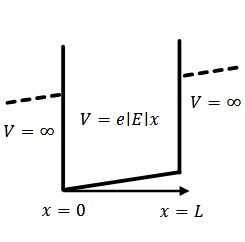
\includegraphics[width=0.25\textwidth]{Tilted Well.png}
\end{figure}

\begin{enumerate}[a)]

\item Write down the WKB quantization condition
$$\frac{1}{\hbar}\int p(x)dx = n\pi$$
for this system. \textit{Note}: this potential has 2 "hard walls".

\color{violet}
The quantization condition for this system is
$$\int_{0}^{L} \sqrt{2m (E - e|E|x)}dx = n\pi\hbar$$
\color{black}

\item Evaluate the integral to obtain an expression in terms of the bound state energies $E_{n}$.

\textit{Note}: you will not be able to solve for $E_{n}$ analytically.

\color{violet}
By defining some $a = \frac{2E}{me|E|}$ such that the integral becomes $\int_{0}^{L} \sqrt{a - x}$. 
\color{black}

\item Using a graphical or numerical method, solve for the three lowest-energy bound states in the potential well for the following parameters:

\begin{itemize}

\item Well width: $L = 1$nm 

\item Electric field magnitude: $|E| = 1.0 \times 10^{8}$ V/m

\end{itemize}

How do these energies compare to the lowest three energies of the infinite square well with a flat well bottom?

\item What effect does introducing an electric field have on the energy levels in the potential well? How would this impact the wavelength of the photons emitted from the quantum well?

\end{enumerate}

\end{enumerate}

\end{document}